% Asset ID: FAS2HookesLawElasticStringsAndSpringsTikZ-001
% Asset type: TikZ diagram
% Source: FM1 Elastic Strings and Springs lesson evidence
% Related lesson section: Section 9 Visual Asset Integration
% Purpose: Precise mathematical diagram for the Hooke's Law lesson.
\documentclass[tikz,border=6mm]{standalone}
\usepackage{amsmath}
\usetikzlibrary{arrows.meta,decorations.pathmorphing}
\begin{document}
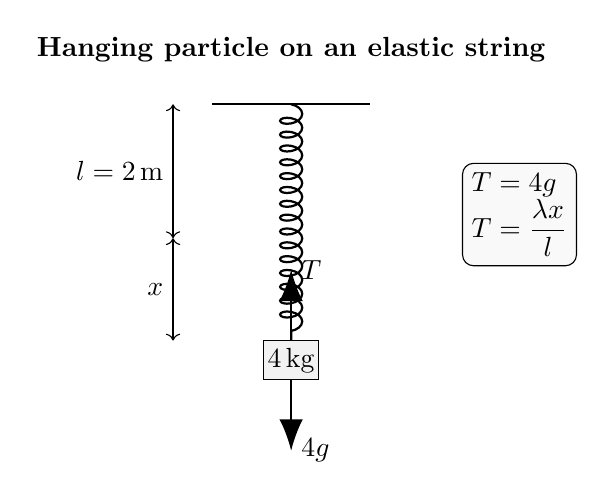
\begin{tikzpicture}[font=\sffamily,force/.style={-{Latex[length=4mm]},draw=black,thick},spring/.style={decorate,decoration={coil,aspect=0.55,segment length=5pt,amplitude=4pt},draw=black,thick}]
\node[font=\bfseries] at (0,0.7) {Hanging particle on an elastic string};
\draw[thick] (-1,0)--(1,0);
\draw[spring] (0,0)--(0,-3);
\draw[fill=gray!10] (-0.35,-3.5) rectangle (0.35,-3);
\node at (0,-3.25) {$4\,\mathrm{kg}$};
\draw[force] (0,-3)--(0,-2.1) node[right] {$T$};
\draw[force] (0,-3.5)--(0,-4.4) node[right] {$4g$};
\draw[<->] (-1.5,0)--(-1.5,-1.7) node[midway,left] {$l=2\,\mathrm{m}$};
\draw[<->] (-1.5,-1.7)--(-1.5,-3) node[midway,left] {$x$};
\node[align=left,draw,rounded corners,fill=gray!5] at (2.9,-1.4) {$T=4g$\\$T=\dfrac{\lambda x}{l}$};
\end{tikzpicture}
\end{document}
